% Copyright 2004 by Till Tantau <tantau@users.sourceforge.net>.
%
% In principle, this file can be redistributed and/or modified under
% the terms of the GNU Public License, version 2.
%
% However, this file is supposed to be a template to be modified
% for your own needs. For this reason, if you use this file as a
% template and not specifically distribute it as part of a another
% package/program, I grant the extra permission to freely copy and
% modify this file as you see fit and even to delete this copyright
% notice. 

\documentclass{beamer}

% There are many different themes available for Beamer. A comprehensive
% list with examples is given here:
% http://deic.uab.es/~iblanes/beamer_gallery/index_by_theme.html
% You can uncomment the themes below if you would like to use a different
% one:
%\usetheme{AnnArbor}
%\usetheme{Antibes}
%\usetheme{Bergen}
%\usetheme{Berkeley}
%\usetheme{Berlin}
%\usetheme{Boadilla}
%\usetheme{boxes}
%\usetheme{CambridgeUS}
%\usetheme{Copenhagen}
%\usetheme{Darmstadt}
\usetheme{default}
%\usetheme{Frankfurt}
%\usetheme{Goettingen}
%\usetheme{Hannover}
%\usetheme{Ilmenau}
%\usetheme{JuanLesPins}
%\usetheme{Luebeck}
%\usetheme{Madrid}
%\usetheme{Malmoe}
%\usetheme{Marburg}
%\usetheme{Montpellier}
%\usetheme{PaloAlto}
%\usetheme{Pittsburgh}
%\usetheme{Rochester}
%\usetheme{Singapore}
%\usetheme{Szeged}
%\usetheme{Warsaw}

\usepackage{amsmath}
\setbeamercovered{transparent}

\usepackage{pifont}% http://ctan.org/pkg/pifont
\newcommand{\cmark}{\ding{51}}%
\newcommand{\xmark}{\ding{55}}%

\usepackage[many]{tcolorbox}
\newtcolorbox{cross}{blank,breakable,parbox=false,
  overlay={\draw[red,line width=1pt] (interior.south west)--(interior.north east);
    \draw[red,line width=1pt] (interior.north west)--(interior.south east);}}

\title{Anomaly detection based on generative adversarial networks for new physics mining at the LHC}

\author{Oliver Knapp \inst{1}}
% - Give the names in the same order as the appear in the paper.
% - Use the \inst{?} command only if the authors have different
%   affiliation.

\institute[Swiss Federal Institute of Technology] % (optional, but mostly needed)
{
  \inst{1}%
  Department of Physics \\
  Swiss Federal Institute of Technology
}
% - Use the \inst command only if there are several affiliations.
% - Keep it simple, no one is interested in your street address.

\date{Semester Project Presentation, 2019}
% - Either use conference name or its abbreviation.
% - Not really informative to the audience, more for people (including
%   yourself) who are reading the slides online

\subject{High Energy Physics}
% This is only inserted into the PDF information catalog. Can be left
% out. 

% If you have a file called "university-logo-filename.xxx", where xxx
% is a graphic format that can be processed by latex or pdflatex,
% resp., then you can add a logo as follows:

% \pgfdeclareimage[height=0.5cm]{university-logo}{university-logo-filename}
% \logo{\pgfuseimage{university-logo}}

% Delete this, if you do not want the table of contents to pop up at
% the beginning of each subsection:
\AtBeginSubsection[]
{
  \begin{frame}<beamer>{Outline}
    \tableofcontents[currentsection,currentsubsection]
  \end{frame}
}

% Let's get started
\begin{document}

\begin{frame}
  \titlepage
\end{frame}

\begin{frame}{Outline}
  \tableofcontents
  % You might wish to add the option [pausesections]
\end{frame}

% Section and subsections will appear in the presentation overview
% and table of contents.
\section{Introduction and Basics}

\begin{frame}{Overview}
  \begin{itemize}
      \item Main goal of LHC: search for deviations from the SM \pause
      \item Typically fully-supervised hypothesis tests (model-dependent) \pause
      \item Alternative: model-independent searches \pause
      \item Cerri et al. proposed anomaly detection using variational autoencoders (VAE) to implement this task \pause
      \item We investigate a GAN based anomaly detector and
      \begin{itemize}
        \pause
        \item benchmark and compare it with VAE
        \pause
        \item demonstrate its effectiveness for offline analysis by simulating a rediscovery of the top quark
      \end{itemize}
  \end{itemize}
\end{frame}

\begin{frame}{Anomaly detection based BSM search}
  \begin{itemize}
      \item<1-> It is expected that BSM events are much rarer compared to SM events $\implies$ Try to isolate rare events (outliers)
      \item<2-> This task belongs to the field of anomaly detection (AD), which can be divided into three categories:
      \begin{itemize}
        \item<3-> Supervised AD $\rightarrow$ requires labeling samples as "normal" or "anomalous" \uncover<4->{\textcolor{red}{\xmark}}
        \item<5-> Semi-supervised AD $\rightarrow$ training set must only contain "normal" samples \uncover<6->{\textcolor{red}{\xmark}}
        \item<7-> Unsupervised AD $\rightarrow$ training set mostly consists of "normal" samples but may contain a small fraction of "anomalous" samples \uncover<8->{\textcolor{green}{\cmark}}
      \end{itemize}
  \end{itemize}
\end{frame}

\subsection{Related Work}

\section{GAN based anomaly detection}

\begin{frame}{Motivating generative adversarial networks}
  \begin{itemize}
      \item<1-> Generative adversarial networks (GANs) have recently been very successful
      \item<2-> Similar to VAE (used by Cerri et al.)
      \item<3-> Both GAN and VAE are replicator neural networks
      \item<4-> Objective is to learn the training set distribution
  \end{itemize}
\end{frame}

\begin{frame}{Generative adversarial networks}
  \begin{itemize}
      \item<1-> Basic idea: two networks compete against each other
      \item<2-> Generator network $G: \mathcal{Z} \rightarrow \mathcal{X}$ learns to generate new samples resembling the training set
      \item<3-> Discriminator network $D:\mathcal{X} \rightarrow [0,1]$ learns to distinguish real samples from the generated ones
      \item<4-> Training = solving saddle point problem
      \begin{equation}
      \underset{G}{\textup{min}}\, \underset{D}{\textup{max}}\, V(D,G),
      \end{equation}
      where
      \begin{equation}
        V(D,G)=\mathbb{E}_{x\sim p_\mathcal{X}}[log\,D(x)] + \mathbb{E}_{z\sim p_\mathcal{Z}}[log\,(1-D(G(z))]
      \end{equation}
      
      \item<5-> Solution has property $p_\mathcal{X}=p_G$
  \end{itemize}
\end{frame}

\begin{frame}{GAN for anomaly detection}
  \begin{itemize}
      \item<1-> Exploit $p_\mathcal{X}\approx p_G$ (after training)
      \item<2-> $\textup{Prob[x \textup{is normal sample}]}=p_\mathcal{X}(x) \approx p_G(x)$
      \item<3-> Problem: $p_G$ is not given explicitly, but can only be sampled from by taking $G(z)$ ($z$ uniformly sampled from latent space $\mathcal{Z}$)
      \item<4-> Instead, we adopt a reconstruction based strategy similar to VAE:
      \begin{equation}
        A(x) \sim \underset{z}{\textup{min}} \; \textup{Loss}_{\textup{reco}}(x, G(z))
      \end{equation}
      \item<5-> Solving the minimization problem (e.g. with gradient descent) is computationally very expensive
  \end{itemize}
\end{frame}

\begin{frame}{ALAD algorithm}
  \begin{itemize}
      \item<1-> Zenati et al. propose to use bidirectional-GANs (BiGAN)
      \item<2-> An encoder network $E: \mathcal{X} \rightarrow \mathcal{Z}$ is simultaneously trained with the generator
      \item<3-> The objective of the encoder is to approximate the inverse of the generator, i.e. $G(E(x))\approx x$
      \item<4-> Achieved by solving the saddle point problem
      \begin{align}
    \underset{G,E}{\textup{min}}\, \underset{D_{xz}}{\textup{max}}\, V(D_{xz},E,G),
\end{align}
with the value function given as
\begin{equation}
\begin{split}
    V(D_{xz},E,G)=& \mathbb{E}_{x\sim p_\mathcal{X}}[log\,D_{xz}(x, E(x))] + \\
    & \mathbb{E}_{z\sim p_\mathcal{Z}}[log\,(1-D_{xz}(G(z), z)]
\end{split}
\end{equation}
  \end{itemize}
\end{frame}

\begin{frame}{ALAD algorithm}
  \begin{itemize}
      \item<1-> Training process does not necessarily converge $\rightarrow$ further modifications needed.
      \item<2-> Add discriminator $D_{xx}$ to enforce cycle consistency $G(E(x))\approx x$
      \item<3-> Add discriminator $D_{zz}$ to regularize latent space
  \end{itemize}
  
  \begin{figure}[!htb]
    \begin{center}
    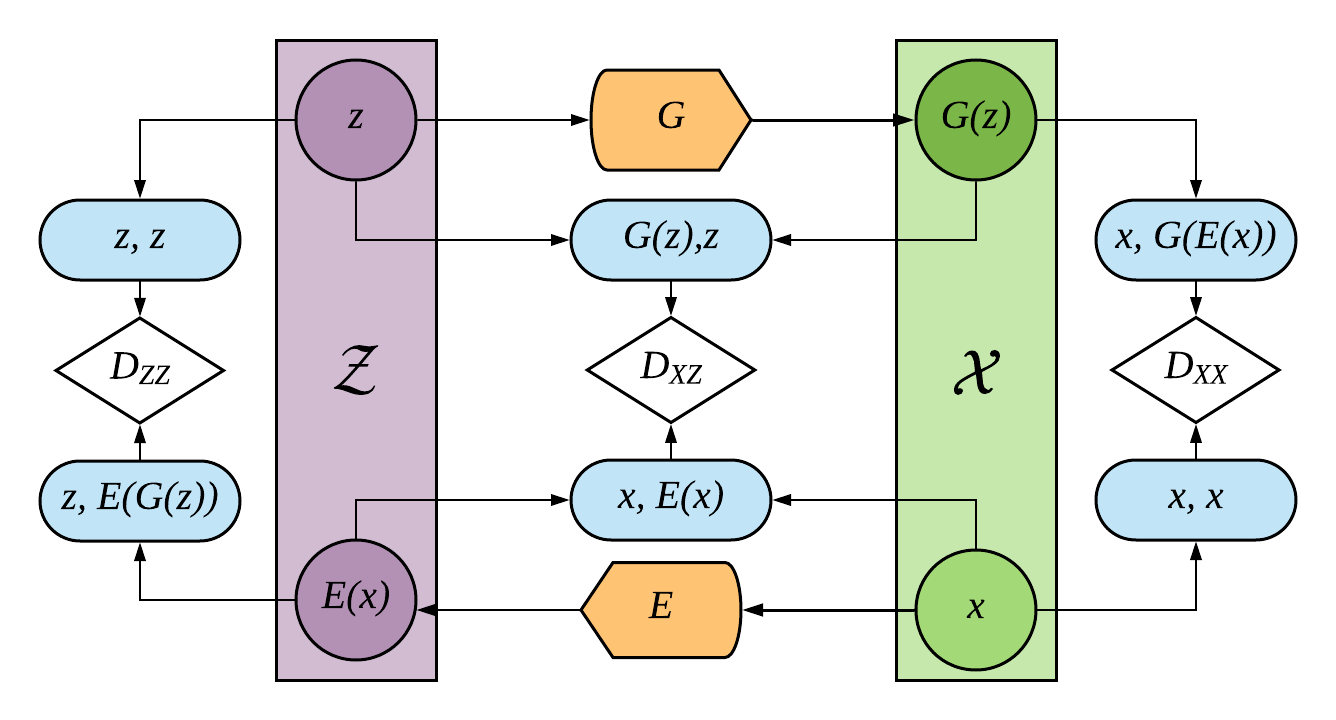
\includegraphics[width=0.7\textwidth]{dladded}
    \caption{Adapted from "Adversarially learned anomaly detection" by Zenati et al.}
    \label{fig:alad}
    \end{center}
  \end{figure}
\end{frame}

\begin{frame}{ALAD anomaly scores}
  \begin{itemize}
      \item<1-> Four proposed anomaly score models
      \item<2-> $L_1$-score: $A(x)=||x-G(E(x))||_{1}$
      \item<3-> $L_2$-score: $A(x)=||x-G(E(x))||_{2}$
      \item<4-> Logits-score: $A(x)=log(D_{xx}(x, G(E(x)))$
      \item<5-> Features-score: $A(x)=||f_{xx}(x,x) - f_{xx}(x, G(E(x)))||_1$, where $f_{xx}(\cdot,\cdot)$ are the activation values in the last hidden layer of $D_{xx}$
  \end{itemize}
\end{frame}

\begin{frame}{Data format}
  \begin{itemize}
      \item<1-> One events recorded by the CMS detector contains $O(10^3)$ particles resulting in $O(10^4)$ parameters
      \item<2-> To reduce dimensionality an event is represented with high-level-features (HLF)
      \item<3-> Jet quantities: $H_T$, $M_J$, $N_J$, $N_b$
      \item<4-> Muon/electron quantities: $p_{T,TOT}^\mu$, $M_\mu$, $N_\mu$, $p_{T,TOT}^e$, $M_e$, $N_e$
      \item<5-> Particle multiplicities: $N_{neu}$, $N_{ch}$, $N_\gamma$
      \item<6-> Missing transverse momentum $p_T^\textup{miss}$
      \item<7-> Selected lepton $\ell$ quantities: $p_T^\ell$, $\eta_\ell$, $q_\ell$, $\textup{IsEle}$, $\textup{Iso}_{ch}^\ell$, $\textup{Iso}_{neu}^\ell$, $\textup{Iso}_{\gamma}^\ell$
      \item Selected lepton and missing system: $M_T$, $p_{T,\parallel}^\textup{miss}$, $p_{T,\perp}^\textup{miss}$
  \end{itemize}
\end{frame}

\subsection{GANs}

\subsection{GANs for anomaly detection}
%naive idea
%ALAD
\subsection{Data format}

\section{ALAD benchmark}
\subsection{Setup}
\subsection{Results}

\section{Top quark rediscovery}
%\subsection{Idea}
%\subsection{Data}
%\subsection{Analysis}

\section{Conclusion}

\begin{frame}{First Slide Title}{Optional Subtitle}
  \begin{itemize}
  \item {
    My first point.
  }
  \item {
    My second point.
  }
  \end{itemize}
\end{frame}

\subsection{Second Subsection}

% You can reveal the parts of a slide one at a time
% with the \pause command:
\begin{frame}{Second Slide Title}
  \begin{itemize}
  \item {
    First item.
    \pause % The slide will pause after showing the first item
  }
  \item {   
    Second item.
  }
  % You can also specify when the content should appear
  % by using <n->:
  \item<3-> {
    Third item.
  }
  \item<4-> {
    Fourth item.
  }
  % or you can use the \uncover command to reveal general
  % content (not just \items):
  \item<5-> {
    Fifth item. \uncover<6->{Extra text in the fifth item.}
  }
  \end{itemize}
\end{frame}

\section{Second Main Section}

\subsection{Another Subsection}

\begin{frame}{Blocks}
\begin{block}{Block Title}
You can also highlight sections of your presentation in a block, with it's own title
\end{block}
\begin{theorem}
There are separate environments for theorems, examples, definitions and proofs.
\end{theorem}
\begin{example}
Here is an example of an example block.
\end{example}
\end{frame}

% Placing a * after \section means it will not show in the
% outline or table of contents.
\section*{Summary}

\begin{frame}{Summary}
  \begin{itemize}
  \item
    The \alert{first main message} of your talk in one or two lines.
  \item
    The \alert{second main message} of your talk in one or two lines.
  \item
    Perhaps a \alert{third message}, but not more than that.
  \end{itemize}
  
  \begin{itemize}
  \item
    Outlook
    \begin{itemize}
    \item
      Something you haven't solved.
    \item
      Something else you haven't solved.
    \end{itemize}
  \end{itemize}
\end{frame}



% All of the following is optional and typically not needed. 
\appendix
\section<presentation>*{\appendixname}
\subsection<presentation>*{For Further Reading}

\begin{frame}[allowframebreaks]
  \frametitle<presentation>{For Further Reading}
    
  \begin{thebibliography}{10}
    
  \beamertemplatebookbibitems
  % Start with overview books.

  \bibitem{Author1990}
    A.~Author.
    \newblock {\em Handbook of Everything}.
    \newblock Some Press, 1990.
 
    
  \beamertemplatearticlebibitems
  % Followed by interesting articles. Keep the list short. 

  \bibitem{Someone2000}
    S.~Someone.
    \newblock On this and that.
    \newblock {\em Journal of This and That}, 2(1):50--100,
    2000.
  \end{thebibliography}
\end{frame}

\end{document}


